\chapter{Introduction}
\label{chp:intro}
\noindent In this Chapter, introduction of \gls{webrtc} and \gls{sip} network will be covered. \gls{sip} is one of the \gls{voip} signaling protocols widely used in current internet telephony service which is also the target telephony network integrated with \gls{webrtc} application system in this thesis.

\section{WebRTC}

\noindent Gmail\footnote{Gmail is a free , advertising-supported email service provided by Google.} video chat became popular in 2008, and in 2011 Google introduced Hangouts\footnote{Google Hangouts is an instant messaging and video chat platform developed by Google, which launched on May 15, 2013 during the keynote of its I/O development conference. It replaces three messaging products that Google had implemented concurrently within its services, including Talk, Google+ Messenger, and Hangouts, a video chat system present within Google+.}, which uses the Google Talk service (as does Gmail). Google bought \gls{gips}, a company which had developed many components required for \gls{rtc}, such as codecs and echo cancellation techniques. Google open sourced the technologies developed by \gls{gips} and engaged with relevant standards bodies at the \gls{ietf} and \gls{w3c} to ensure industry consensus. In May 2011, Ericsson built the first implementation of \gls{webrtc}.

\subsection{What is WebRTC ?}

\noindent \gls{webrtc} is an industry and standards effort to put real-time communications capabilities into all browsers and make these capabilities accessible to web developers via standard \gls{html5} tags and JavaScript \gls{api}s. For example, consider functionality similar to that offered by Skype\footnote{Skype is a freemium voice-over-IP service and instant messaging client, currently developed by the Microsoft Skype Division.\cite{wiki:skype}}. but without installing any software or plug-ins. For a website or web application to work regardless of which browser is used, standards are required. Also, standards are required so that browsers can communicate with non-browsers, including enterprise and service provider telephony and communications equipment\cite{inbook:rtc-intro}.

\par With the rapidly development of internet, more and more communication traffic is moving to web from the traditional telephony network. And in the recent decade, \gls{voip} network services are growing to the peek of the market capacity. Solution to integrate \gls{webrtc} and existing \gls{voip} network is the right approach the trend of the internet communication requirement.

\subsection{WebRTC Network Structure}

\noindent In the Figure\ref{fig:webrtc_network_finCandidate}\cite{html5rock:webrtc} shows how the \gls{ice} framework\footnote{ICE is a framework for connecting peers, such as two video chat clients.\cite{wiki:ice}} to find peer candidate through \gls{stun} server and its extension \gls{turn} server.

\begin{figure}
	\centering
    	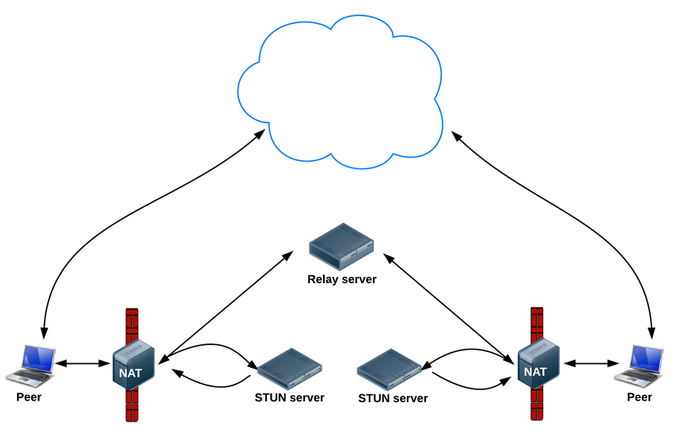
\includegraphics[height=0.30\textheight,natwidth=610,natheight=642]{figs/webrtc_network_finCandidate.png}
  	\caption{\gls{webrtc} Network: Finding connection candidates\cite{html5rock:webrtc}}
  	\label{fig:webrtc_network_finCandidate}
\end{figure} 

\begin{figure}
	\centering
    	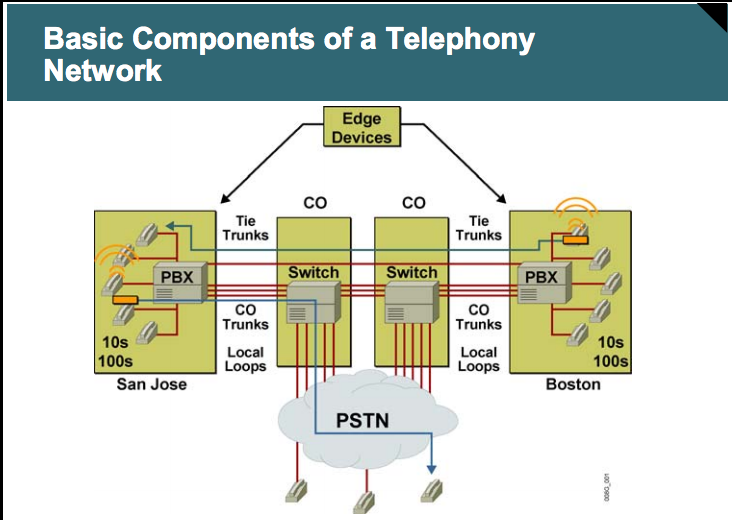
\includegraphics[height=0.40\textheight,natwidth=610,natheight=642]{figs/telephony_network.png}
  	\caption{Traditional Telephony Network}
  	\label{fig:telephony_network}
\end{figure}

\par Initially, \gls{ice} tries to connect peers directly, with the lowest possible latency, via \gls{udp}. In this process, \gls{stun} servers have a single task which is to enable a peer behind a \gls{nat} to find out its public address and port. If \gls{udp} fails, \gls{ice} tries \gls{tcp} (first \gls{http}, then \gls{https}). If direct connection fails in particular, because of enterprise \gls{nat} traversal and firewalls \gls{ice} uses an intermediary (relay) \gls{turn} server. In other words, \gls{ice} will first use \gls{stun} with \gls{udp} to directly connect peers and, if that fails, will fall back to a \gls{turn} relay server. The expression 'finding candidates' refers to the process of finding network interfaces and ports.\cite{html5rock:webrtc}

\par The difference and usage of \gls{stun} server and \gls{turn} server will be discussed more detail in Chapter \ref{chp:sys_deploy}.

\par \gls{webrtc} needs server to help users discover each other and exchange 'real world' details such as names. Then \gls{webrtc} client applications (peers) exchange network information. After that, peers exchange data information about media such as video format and resolution. Finally, \gls{webrtc} client applications can traverse \gls{nat} gateways and firewalls.

\par Compare to the traditional telephony network which is shown in Figure\ref{fig:telephony_network}\cite{web:teleVSvoip}, the main difference between these two communication network is that \gls{webrtc} is \gls{p2p} communication in \gls{stun} server scenario, after the signaling between end-peers, the media data are exchanged directly between two peers. However, in the traditional telephony, all the media data are transferred to \gls{pbx} and switches regarding to \gls{pstn}\footnote{The PSTN consists of telephone lines, fiber optic cables, microwave transmission links, cellular networks, communications satellites, and undersea telephone cables, all interconnected by switching centers, thus allowing any telephone in the world to communicate with any other. Originally a network of fixed-line analog telephone systems, the PSTN is now almost entirely digital in its core network and includes mobile and other networks, as well as fixed telephones.\cite{wiki:pstn}} then reach the other side of the peer. Even in \gls{turn} server scenario for \gls{webrtc}, the media stream is only relaying to the \gls{turn} then directly transfer to another peer, no switches involved.

\subsection{WebRTC Implementation Steps}

\begin{figure}
	\centering
    	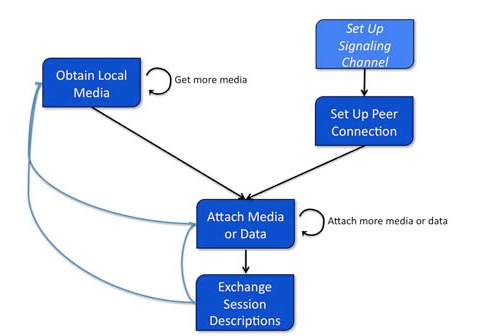
\includegraphics[width=0.80\textwidth,natwidth=610,natheight=642]{figs/webrtcApis.png}
  	\caption{WebRTC \gls{api} View with Signaling\cite{inbook:rtc-apis}}
  	\label{fig:webrtc_4steps}
\end{figure}

\noindent There are four main steps to implement a \gls{webrtc} session shown in Figure \ref{fig:webrtc_4steps}. The browser client need to obtain local media first, then set up a connection between the browser and the other peer through some signaling, after that attach the media and data channels to the connection, afterwards exchange the session description from each other. Then the media stream will automatically exchange through the real-time peer to peer media channel.

\par Each step shown in the Figure \ref{fig:webrtc_4steps} is implemented by some \gls{webrtc} \gls{api}s. More detail about how to use these \gls{webrtc} \gls{api}s to implement these steps will be covered in Chapter \ref{chp:sys_imp}. The \gls{webrtc} architecture is shown in Figure \ref{fig:webrtc_api_arch}, the main focus in this thesis will be Web \gls{api} part and transport part because Web \gls{api} is the tool to implement the \gls{webrtc} application and transport part is the key for \gls{webrtc} application to communicate with application server, media server and any other end peer in the system. 

\begin{figure}
	\centering
    	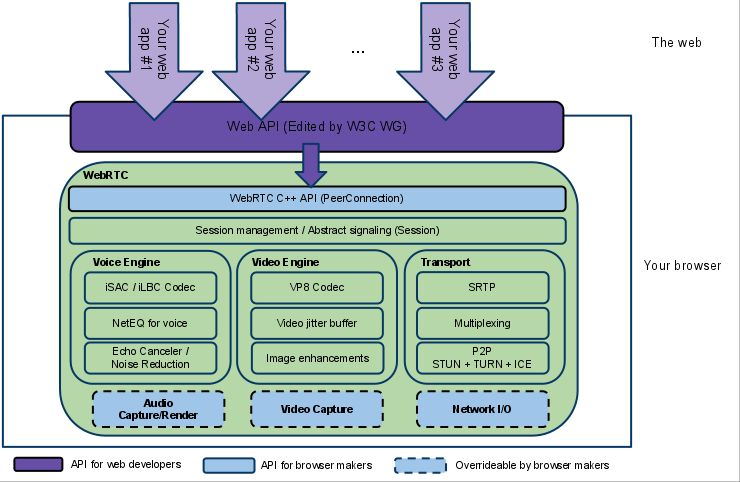
\includegraphics[width=0.80\textwidth,natwidth=610,natheight=642]{figs/WebRTCapiPic.png}
  	\caption{\gls{webrtc} architecture \cite{org:webrtc}}
  	\label{fig:webrtc_api_arch}
\end{figure}

\par Besides \gls{webrtc} \gls{api}s, signaling is the other important factor in the system. \gls{webrtc} uses \textit{RTCPeerConnection} (more about this \gls{api} will be discussed in Chapter \ref{chp:sys_imp}) to communicate streaming data between browsers, but also needs a mechanism to coordinate communication and to send control messages, a process known as signaling. Signaling methods and protocols are not specified by \gls{webrtc} by Google in purpose, then signaling is not part of the \textit{RTCPeerConnection} \gls{api} which can be decide how to implemented based on different project scenario.

\par Instead, \gls{webrtc} app developers can choose whatever messaging protocol they prefer, such as \gls{sip} or \gls{xmpp}, and any appropriate duplex (two-way) communication channel. The prototype application in this thesis will use WebSocket\footnote{WebSocket is a protocol providing full-duplex communications channels over a single TCP connection.\cite{wiki:websocket}} as signaling between \gls{webrtc} browser end point and keep use \gls{sip} as signaling for \gls{sip} end point (mobile/fixed phone based on \gls{pstn} in this case).

\noindent Signaling is used to exchange three types of information in \gls{webrtc}\cite{html5rock:webrtc}:

\begin{itemize}[topsep=-1em,parsep=0em,itemsep=0em]
 \item Session control messages: to initialize or close communication and report errors.
 \item Network configuration: to the outside world, the computer's IP address and port.
 \item Media capabilities: the codecs and resolutions can be handled by the browser and the browser it wants to communicate with.
\end{itemize}

\par The exchange of information via signaling must have completed successfully before peer-to-peer streaming can begin. For the prototype application in this thesis, the signaling has two mechanisms, one is for \gls{webrtc} browser clients and the other is for \gls{sip} clients, it will be explained in Chapter \ref{chp:sys_imp}.

\section{SIP}
\noindent The prototype application in this thesis will be integrated with \gls{pstn} through \gls{sip} server. Therefore the application server implemented in this system will use \gls{sip} as signaling to communicate with \gls{sip} server to handle the signaling configuration with mobile/fixed phone end-point.

\subsection{What is SIP ?}
\noindent The \gls{sip} is a signaling communication protocol, widely used for controlling multimedia communication sessions such as voice and video calls over \gls{ip} networks.

\par The protocol defines the messages that are sent between endpoints which govern establishment, termination and other essential elements of a call. \gls{sip} can be used for creating, modifying and terminating sessions consisting of one or several media streams. \gls{sip} can be used for two-party (unicast) or multiparty (multicast) sessions. Other \gls{sip} applications include video conferencing, streaming multimedia distribution, instant messaging, presence information, file transfer, fax over \gls{ip} and online games.\cite{wiki:sip}

\par \gls{sip} works in conjunction with several other application layer protocols that identify and carry the session media. Media identification and negotiation is achieved with the \gls{sdp}. It is different key filed format than the \gls{webrtc} \gls{sdp}. For the transmission of media streams (voice, video) \gls{sdp} typically employs the \gls{rtp} or \gls{srtp}. For secure transmissions of \gls{sip} messages, the protocol can be encrypted with \gls{tls}.

\subsection{SIP Network Elements}
\noindent In normal \gls{sip} network, \gls{sip} defines user-agents as well as several types of server network elements. Two \gls{sip} endpoints can communicate without any intervening \gls{sip} infrastructure. However, this approach is often impractical for a public service, which needs directory services to locate available nodes on the network. In the system implemented of this thesis, the application server will play the roles as 'User Agent', 'Registrar' and 'Gateway' elements in the \gls{sip} network.

\noindent \textbf{User Agent}\cite{wiki:sip}:
\par A \gls{sip} \gls{ua} is a logical network end-point used to create or receive \gls{sip} messages and thereby manage a \gls{sip} session. A \gls{sip} \gls{ua} can perform the role of a \gls{uac}, which sends \gls{sip} requests, and the \gls{uas}, which receives the requests and returns a \gls{sip} response. These roles of \gls{uac} and \gls{uas} only last for the duration of a \gls{sip} transaction.

\noindent \textbf{Registrar}\cite{wiki:sip}:
\par A registrar is a \gls{sip} endpoint that accepts REGISTER requests and places the information it receives in those requests into a location service for the domain it handles. The location service links one or more \gls{ip} addresses to the \gls{sip} \gls{uri} of the registering agent. The \gls{uri} uses the sip: scheme, although other protocol schemes are possible, such as tel:. More than one user agent can register at the same \gls{uri}, with the result that all registered user agents receive the calls to the \gls{uri}.

\noindent \textbf{Gateway}\cite{wiki:sip}:
\par Gateways can be used to interface a \gls{sip} network to other networks, such as the \gls{pstn}, which use different protocols or technologies. In the prototype application, the application server is the gateway to interface a \gls{webrtc} WebSocket network. The working process will be covered in Chapter \ref{chp:sys_imp}.

\subsection{SIP messages}
\noindent Since the application server in this system will be used as \gls{sip} \gls{ua} and \gls{sip} Gateway, it will send \gls{sip} message requests to \gls{sip} server and receive \gls{sip} message requests from the \gls{sip} server.

\par One of the wonderful things about \gls{sip} is that it is a text-based protocol modeled on the request/response model used in \gls{http}. This makes it easy to debug because the messages are easy to construct and easy to see.  Contrasted with H.323\footnote{H.323 is a recommendation from the ITU Telecommunication Standardization Sector (ITU-T) that defines the protocols to provide audio-visual communication sessions on any packet network. The H.323 standard addresses call signaling and control, multimedia transport and control, and bandwidth control for point-to-point and multi-point conferences.\cite{wiki:h323}}, SIP is an exceedingly simple protocol.  Nevertheless, it has enough powerful features to model the behavior of a very complex traditional telephone \gls{pbx}.\cite{networkworld:sip}

\par There are two different types of \gls{sip} messages: requests and responses. The first line of a request has a method, defining the nature of the request, and a Request-\gls{uri}, indicating where the request should be sent.The first line of a response has a response code.

\noindent For sip requests, regarding to RFC 3261\cite{rfc:3261}, the application server in the system will use following \gls{sip} messages:

\begin{itemize}[topsep=-1em,parsep=0em,itemsep=0em]
 \item \textbf{REGISTER:} Used by a \gls{ua} to indicate its current \gls{ip} address and the \gls{url}s for which it would like to receive calls.
 \item \textbf{INVITE:} Used to establish a media session between user agents.
 \item \textbf{ACK:} Confirms reliable message exchanges.
 \item \textbf{CANCEL:} Terminates a pending request.
 \item \textbf{BYE:} Terminates a session between two users in a conference.
\end{itemize}

\noindent The \gls{sip} response types defined in RFC 3261 will be listened by application server in the following response codes\cite{wiki:sip_response_codes}:

\begin{itemize}[topsep=-1em,parsep=0em,itemsep=0em]
 \item \textbf{100 Trying:} Extended search being performed may take a significant time so a forking proxy must send a 100 Trying response.
 \item \textbf{180 Ringing:} Destination user agent received INVITE, and is alerting user of call.
 \item \textbf{200 OK:} Indicates the request was successful.
 \item \textbf{400 Bad Request:} The request could not be understood due to malformed syntax.
 \item \textbf{401 Unauthorized:} The request requires user authentication. This response is issued by \gls{uas}s and registrars.
 \item \textbf{408 Request Timeout:} Couldn't find the user in time. The server could not produce a response within a suitable amount of time, for example, if it could not determine the location of the user in time. The client MAY repeat the request without modifications at any later time.
 \item \textbf{480 Temporarily Unavailable:} Callee currently unavailable.
 \item \textbf{486 Busy Here:} Callee is busy.
\end{itemize}

\par By listening these \gls{sip} response, the application will send requests to either \gls{webrtc} browser client or \gls{sip} client to play as the gateway role in the system. This gateway mechanism will be introduced in Chapter \ref{chp:sys_design}.

\section{Prototype System Working Flow}

\noindent The main purpose of this thesis is to make unified communication solution with \gls{webrtc} technology.

\par To connect with the traditional telephony network, the \gls{voip} system bridges the \gls{pstn} and the \gls{ip} network. \gls{voip} systems employ session control and signaling protocols to control the signaling, set-up, and tear-down of calls. They transport audio streams over \gls{ip} networks using special media delivery protocols that encode voice, audio, video with audio codecs, and video codecs as Digital audio by streaming media. In the prototype system, \gls{sip} signaling is used because of its widely usage and current target \gls{pstn} has \gls{sip} server support.

\begin{figure}
	\centering
    	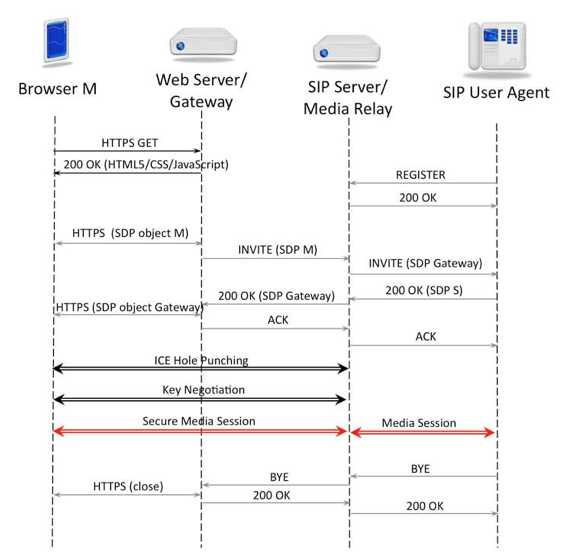
\includegraphics[width=0.60\textheight,natwidth=610,natheight=642]{figs/system_work_flow.png}
  	\caption{Prototype System Working Diagram \cite{inbook:sys_work_diagram}}
  	\label{fig:sys_work_diagram}
\end{figure}

\par The Figure \ref{fig:sys_work_diagram} shows the basic working flow of the prototype system. The Web Server/ Gateway is the application server in the prototyep system, it mainly bridges the \gls{webrtc} browser client with other \gls{webrtc} clients and the \gls{sip} network. The \gls{sip} server bridges the \gls{sip} network and \gls{pstn} network or traditional telephony network. And also the Media Relay server relay all the media stream from different end clients. In the prototype system, there is another media server besides the media relay function provided by \gls{sip} server because the media server needs to handle different media \gls{sdp} in signalings which are \gls{webrtc} \gls{sdp} and \gls{sip} \gls{sdp}. The media server used in the prototype system is provided by Dialogic, the Network Fuel company, which is called PowerMedia XMS v2.1\footnote{PowerMedia XMS is pre-integrated with a variety of application servers and signaling gateways with HTTP-to-SIP (H2S) functionality and rapidly integrates with others using its web API or standard interfaces.}. PowerMedia XMS acts as a WebRTC Media Gateway to mediate WebRTC media-plane differences from those of typical existing VoIP networks including encryption interworking, transcoding, and client-based NAT traversal support. The reason to use this media server is to avoid hard-code transition between \gls{webrtc} \gls{sdp} and \gls{sip} \gls{sdp}. Then the end client no matter is a \gls{webrtc} client or a \gls{sip} client, they will communicate with the same signaling client in their aspect.

\par Moreover, since the media server is used in this case, during the multiple end-point conversation, each end-point will only exchange their media stream to the single end-point on the media server (PowerMedia XMS server), it will make light client and centralized media server control. The benefit of this system architecture will be discussed more in the Chapter \ref{chp:sys_design}.

\par Therefore, in the Figure \ref{fig:sys_work_diagram}, all the end point keep using their own original signaling protocol to communicate with different servers of the prototype system in order to reach different scope end point.